%********************************************************************************************
%								COMANDOS ÚTILES PARA LATEX EN ESTE TP							
%
%	\ : espacio simple
%	\\ : nueva línea
%	\par : va a la línea de abajo y deja sangría
%	\vspace{##tamaño en pt##} o \vspace{\baselineskip} en general:
%								 para dejar un espacio vertical
%	\textbf{text} :text en negrita
%	\textit{text} :text en itálica
%
% GRAFICOS CENTRADOS:
%	\begin{center}
%		\includegraphics[width=\textwidth]{./img/##ruta imagen (no hace falta extension)##}
%	\end{center}
%		--> se pueden agregar atributos como scale por si se hace muy grande
%
% TABLAS CENTRADAS:
%	\begin{center}
%	\begin{tabular}{|c|c|}
%	\hline
%	\ \textbf{Programa} & \textbf{Ticks} \\
%	\hline
%		ASM & 675127609 \\
%	\hline
%	\end{tabular}
%	\end{center}
%
% ALGORITMOS (EN VARIOS LENGUAJES):
% \begin{lstlisting}
%	void sumoDiez(int &num)
%	{
%	    num += 10;
%	}
%	
%	int main()
%	{
% 	   int i;
%	    int numeroAProcesar = 20;
%	    for (i = 0; i < 50; i++)
%	    {
%	        sumoDiez(numeroAProcesar);	//Proceso el numero en cada ciclo
%	    } 
%	    return 0;
%	}
%	\end{lstlisting}
%
% para info sobre todo lo que tiene el package detallado:
% http://en.wikibooks.org/wiki/LaTeX/Source\_Code\_Listings
%
%********************************************************************************************

\documentclass[10pt,a4paper]{article}
\usepackage[utf8]{inputenc} % para poder usar tildes en archivos UTF-8
\usepackage[spanish]{babel} % para que comandos como \today den el resultado en castellano
\usepackage{a4wide} % márgenes un poco más anchos que lo usual
\usepackage[conEntregas]{caratula}
\usepackage{amssymb}
\usepackage{fancybox}
\usepackage[usenames,dvipsnames]{color}
\usepackage{hyperref}
\usepackage{listings}
\usepackage{color}
\usepackage[table]{xcolor}
\usepackage{amsmath}
\usepackage{float}
\usepackage{pdflscape}
\usepackage{chngpage}
\usepackage{lscape}

\hypersetup{
    colorlinks,
    citecolor=black,
    filecolor=black,
    linkcolor=black,
    urlcolor=black
}

\lstdefinestyle{customc}{
  belowcaptionskip=1\baselineskip,
  breaklines=true,
  frame=L,
  xleftmargin=\parindent,
  language=C,
  showstringspaces=false,
  basicstyle=\footnotesize\ttfamily,
  keywordstyle=\bfseries\color{green!40!black},
  commentstyle=\itshape\color{purple!40!black},
  identifierstyle=\color{blue},
  stringstyle=\color{orange},
}

\lstset{escapechar=@,style=customc}

\begin{document}

\titulo{Trabajo Práctico 2}
\subtitulo{Rutas en internet}

\fecha{\today}

\materia{Teoría de las Comunicaciones}
\grupo{}

\integrante{Barbeito, Nicolás}{147/10}{nicolasbarbeiton@gmail.com}
\integrante{Garassino, Agustín Javier}{394/12}{ajgarassino@gmail.com}
\integrante{Vileriño, Silvio}{106/12}{svilerino@gmail.com}

\maketitle

\tableofcontents
\newpage
\section{Introducción}
En este trabajo pr\'actico ejercitaremos las nociones del nivel de transporte estudiadas en la materia a
través del análisis de un protocolo PTC implementado por la c\'atedra. Este protocolo se encuentra basado en TCP, pero simplificado. Es bidireccional, orientado a conexi\'on y confiable.\\

El objetivo es generar un escenario de an\'alisis en el contexto de una red local, de cliente-servidor en el cual el cliente env\'ia datos y el servidor solo los reconoce. En una etapa inicial, realizaremos diversos experimentos y observacion sobre esos resultados para fijar valores optimos para los par\'ametros $\alpha$ y $\mathcal{B}$ que optimizan el c\'alculo de RTO (Retransmission Time Out).\\

Finalmente, analizaremos de qu\'e manera afectan los efectos de red (delay y p\'erdida de paquetes) a la aproximacion del RTO con los parametros de la etapa inicial fijos.
\section{Desarrollo}
\subsection{Implementación de traceroute}
En esta sección explicaremos como fue realizada la herramienta en python que realiza el \texttt{traceroute}.
\subsubsection{Envio de paquetes con ttl incremental}
Utilizamos el protocolo \texttt{ICMP} y la tecnica de \texttt{TTL incrementales} para obtener los hops intermedios de origen a destino, esta tecnica consiste en enviar paquetes \texttt{ICMP} con ttl en un rango creciente, comenzando en 1, y al recibir una respuesta, dependiendo el tipo de respuesta ir armando la ruta, particularmente si la respuesta es \textbf{Time Exceeded}, quiere decir que el ttl del paquete se agoto en camino y obtenemos un hop intermedio de la direccion origen del paquete de la respuesta de \texttt{ICMP}. Si la respuesta es \textbf{Echo Reply}, quiere decir que el host destino fue alcanzado. El incremento del \texttt{TTL} continua en cada iteración hasta o bien llegar al host destino, o bien llegar a un limite de TTL, usualmente 30 saltos en el traceroute de linux, limite que adoptamos para nuestra herramienta.
\subsubsection{Control de hops sin respuesta - Timeout}
Puede ocurrir que para cierto \texttt{TTL} el hop correspondiente no conteste, es por esto que agregamos un \texttt{timeout} asociado a la petici\'on. Luego de este tiempo, el intento con dicho \texttt{TTL} es descartado, marcado el hop como desconocido y se procede a incrementar el \texttt{TTL} y continuar con el ciclo de la traza.
\subsubsection{Medicion del RTT}
Scapy nos provee de ciertos campos temporales en los paquetes, utilizamos estos campos para determinar el tiempo \texttt{Round trip time} o \texttt{Tiempo de ida y vuelta}, en los paquetes de envio y respuesta de la peticion, hay campos indicando el \texttt{Unix Time} en el que fueron enviados y recibidos, correspondientemente, al realizar la resta entre ellos, obtenemos la medicion que buscabamos y al multiplicarla por 1000 obtenemos el tiempo en milisegundos.

\subsection{Informacion obtenida de hops}
Para refinar el análisis, como mencionamos en la introducción, se utilizaron APIs para obtener \texttt{metadatos} acerca de los hops con IP descubierta.

\subsubsection{Reverse DNS Lookup}
Utilizamos el \texttt{Servicio Web} situado en \texttt{http://api.statdns.com/x/<IpAddress>} para resolver los nombres de host de los hop a partir de su direccion IP.

\subsubsection{IP Geolocalization Lookup}
Utilizamos el \texttt{Servicio Web} situado en \texttt{http://freegeoip.net/json/<IpAddress>} para obtener datos de posición geografica de los hops utilizando su dirección IP.

\subsection{Problemas surgidos durante el desarrollo}
\subsubsection{Hops con $RTT_i$ negativo}
Si pensamos a internet como un grafo y los hosts origen y destino como 2 nodos, la traza es el camino entre origen y destino en el grafo, si pensamos que el \texttt{TTL} restringe la cantidad de saltos entre nodos consecutivos que pueden darse a partir del host origen, uno esperaria que el \texttt{RTT} fuera creciente, dado que es acumulativo. Pero al haber varias rutas posibles, diferente congestion a cada instante, diferentes tiempos de encolamiento a cada instante, y otras variables, es posible que en cada pedido el camino no sea el mismo. Esto produce que la medicion de \texttt{RTT} incrementando los \texttt{TTL} no sea creciente.\\

Al momento de calcular los $RTT_i = RTT_{(acum, i)} - RTT_{(acum, i-1)}$ de cada hop la situación explicada arriba puede producir \texttt{RTT incrementales} negativos. Por lo general los nodos distinguidos \textbf{tienen una variación importante de RTT acumulado y no son afectados usualmente por este problema}, de forma que no implementamos ninguna soluci\'on a este problema porque no nos afecta en los resultados que buscamos.

\subsubsection{Hops sin un hop inmediato anterior valido}
Otro problema surge al calcular $RTT_i = RTT_{(acum, i)} - RTT_{(acum, i-1)}$, 
el hop $i-1$ puede no existir, o ser desconocido. En el primer caso, coincide que $RTT_1 = RTT_{(acum, 1)}$ asi que no hay mayores inconvenientes. En caso de ser desconocido el hop anterior, asumiendo que el primer hop, usualmente el gateway del host origen es siempre descubierto, el enfoque utilizado para solucionar este problema fue iterar hacia atras desde el i-esimo hop, y realizar el calculo $RTT_i = RTT_{(acum, i)} - RTT_{(acum, j)}$, donde $j$ es el indice del primer hop detr\'as del i-esimo hop. El problema que trae esto, es que agrupamos hops desconocidos como uno solo, lo que nos va a afectar el descubrimiento de hops distinguidos, dando falsos positivos. Una segunda iteración sobre este enfoque fue simular un RTT equitativo entre todos los hops intermedios ocultos entre el i-ésimo y el j-ésimo hop y asignarle $RTT_i = \frac{RTT_{(acum, i)} - RTT_{(acum, j)}}{cant. hops salteados}$ a cada hop intermedio entre los hops j e i. Finalmente utilizamos esta segunda iteración de la solución para nuestro análisis.

\subsubsection{Varias iteraciones para descubrir rutas y rtt promedio}
Para el descubrimiento de varias rutas y rtt promediado, habiamos pensado en enviar, para cada TTL incremental, un conjunto de requests ICMP a destino, y del conjunto de IPs que respondieran, quedarnos con la IP con mayor frecuencia de aparicion en dicho conjunto, llamemosla IP representante, y para dicha IP, calcular el promedio de los RTT de los requests asociados a esas respuestas. Luego de varios experimentos, nos dimos cuenta que usualmente, para pruebas corridas con pausas pequeñas de tiempo entre ellas, las rutas no variaban y los RTT variaban de forma despreciable, por lo cual decidimos no implementar esto y quedarnos simplemente con el algoritmo basico original de traceroute que funciono bien para todos los experimentos realizados.

\subsubsection{TCPTraceroute para mejorar descubrimiento de hops}
Para intentar disminuir la cantidad de nodos desconocidos, realizamos una prueba enviando paquetes TCP y UDP adaptando las condiciones de terminacion del algoritmo de traza, los resultados obtenidos fueron identicos a las pruebas realizadas con ICMP con lo cual no avanzamos por este camino.

\subsection{Estadísticas y Nodos distinguidos}
Para la detección de nodos distinguidos en la ruta calculamos una serie de estimadores estadisticos.
\subsubsection{Promedio y Desv. Estandar del $RTT_i$}
Al final de la traza, se calcula el promedio y la desviacion estandar del $RTT incremental$ de cada hop en la traza.
\subsubsection{Cálculo de ZScore para cada hop}
Realizando el cálculo $Zrtt_i = \frac{RTT_i - RTT_{prom}}{RTT_{stdev}}$ asignamos un puntaje signado a cada hop, si $Zrtt_i$ es negativo, se encuentra por debajo de la media, si es positivo, se encuentra por encima de la media.

\subsubsection{Eleccion emp\'irica del umbral para deteccion de nodos distinguidos}
Tomamos un umbral arbitrario $\lambda=\frac{1}{2}$, todos los hops que se encuentren con puntaje por encima de este umbral, son considerados distinguidos. Dado que obtuvimos buenos resultados con este umbral, no vimos la necesidad de ajustarlo.

\subsection{Gr\'aficos y an\'alisis realizados}
Para los experimentos realizados a ciertos hosts de distintos continentes se presenta la informacion con las siguientes herramientas.
\begin{itemize}
	\item \texttt{Tabla de hops de la traza: }
	Se muestra una tabla informando los hops entre origen y destino, con el \texttt{RTT acumulado}, el \texttt{RTT incremental} y el \texttt{zscore} de cada hop, y donde es posible, la resolución del \texttt{host-name} y la \texttt{geolocalización} del host.

	\item \texttt{Distribución de $RTT_i$: }
		Se muestra un gráfico de barras donde el eje x indica las IP de los hops y en el eje Y de muestra una barra indicando el \texttt{RTT incremental} entre dicho hop y el anterior.
	\item \texttt{Distribución de $RTT_{ttl}$ acumulado: }
		En este grafico mostramos de izquierda a derecha, los hops en orden desde origen a destino y en el eje Y el \texttt{RTT acumulado} desde orígen hasta este hop.
	\item \texttt{Distribucion de $ZScore_i$: }
		Para cada hop en el eje x, en este gráfico, mostramos en el eje Y una barra indicando el puntaje estandar otorgado a este hop.
\end{itemize}

\subsubsection{Traza sobre el planisferio}
Con el fin de mostrar de forma clara los datos geograficos recolectados con la API mencionada en secciones anteriores, utilizamos una libreria de python que grafica, sobre un planisferio, un punto de tamaño variable segun el score asignado por cada hop de la traza y un arco entre los hops. Esperamos que los nodos submarinos obtenidos de forma estadistica utilizando el puntaje estandar correspondan con los arcos denotando los enlaces submarinos.

\section{Experimentacion}
\subsection{www.unsw.edu}

Con el fin de probar la herramienta implementada para este trabajo, y analizar el funcionamiento del Z-Score como medida para hallar nodos distinguidos dentro de una red, se envió un paquete ICMP con destino al sitio web de la University of New South Wales, ubicada en Australia. El experimento se realizó dentro de los laboratorios de la facultad, al igual que los siguientes que se presentarán en este trabajo práctico, en consecuencia esperamos que el calculo del puntaje nos permita discernir al menos un salto de mayor importancia con respecto a los otros, por ejemplo un salto transoceánico. En primer lugar podemos observar el recorrido realizado por el paquete en el siguiente mapa:

\begin{landscape}
\begin{figure}[H]
  \centering	
	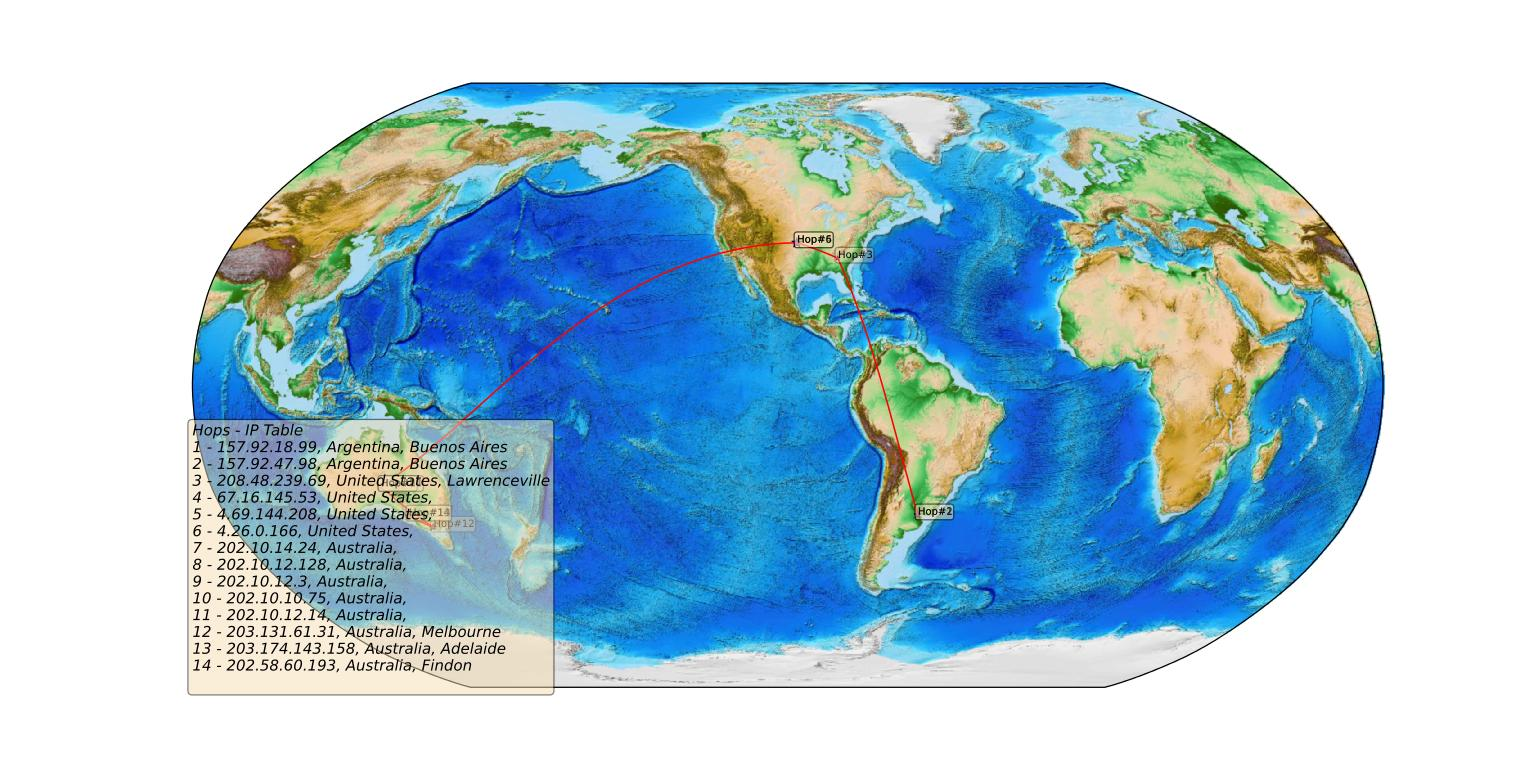
\includegraphics[scale=0.5]{../australia-experiment/figure_1.jpeg}
  \caption{Planisferio el viaje realizado por el paquete resaltado en rojo.}
	\label{fig:histo-src-sitiotrabajo}
\end{figure}
\end{landscape}

Como se puede observar se halla un salto de los Estados Unidos a Australia entre el sexto y septimo hop. Si el Z-Score cumple con su objetivo de la forma esperada, este será resaltado como un \textit{hop} de mayor importancia con respecto a los otros. Veamos que sucede con el \textit{RTT}, que es esperable aumente de manera significativa luego de este salto. El primero del siguiente par de gráficos representa el RTT entre dos host consecutivos, mientras que el segundo representa el acumulado a medida que el paquete se acerca a su destino: 

\begin{figure}[H]
  \centering	
	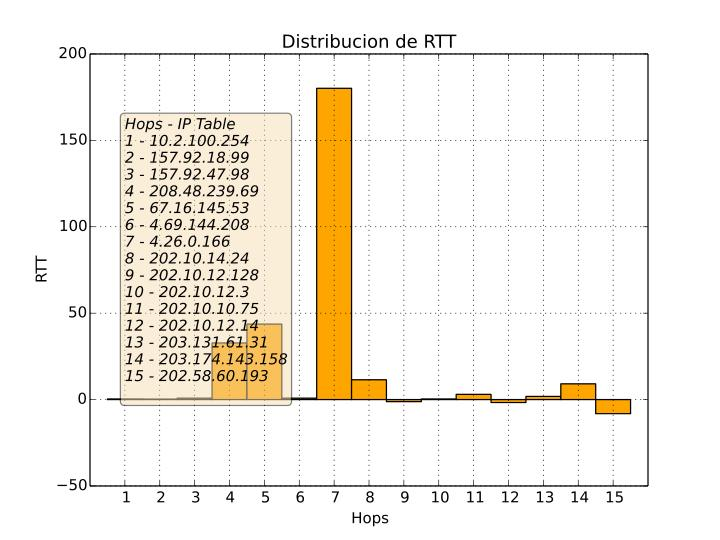
\includegraphics[scale=0.5]{../australia-experiment/bar_rtt.jpeg}
  \caption{RTT entre dos hops consecutivos medido en milisegundos.}
	\label{fig:histo-src-sitiotrabajo}
\end{figure}

\begin{figure}[H]
  \centering	
	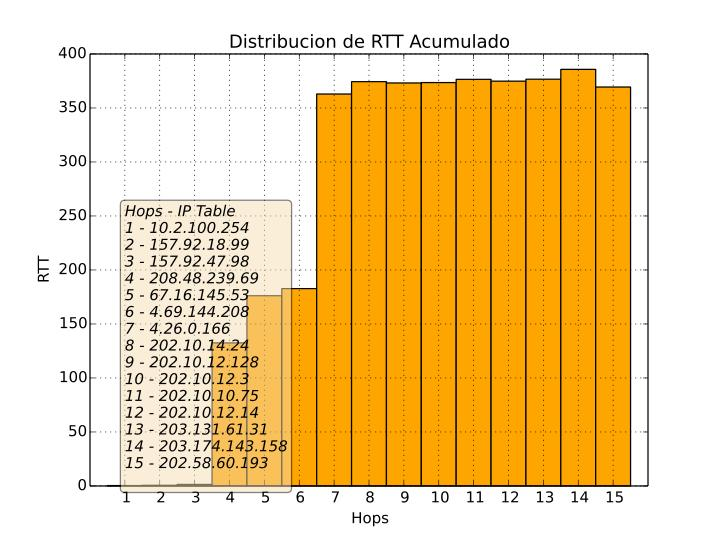
\includegraphics[scale=0.5]{../australia-experiment/bar_rtt_acum.jpeg}
  \caption{RTT acumulado del paquete a medida que avanza en su camino hacia Australia.}
	\label{fig:histo-src-sitiotrabajo}
\end{figure}

Finalmente, presentamos los resultados obtenidos con el Z-Score a partir de los valores obtenidos con la herramienta de \textit{traceroute}. Como se puede ver en el gráfico, la IP distinguida corresponde con el último nodo antes del salto transoceánico con destino a Australia. El resto de los valores o bien son negativos, o no parecen llegar a estar asociados a un nodo representativo del \textit{hop} debido a su reducido puntaje con respecto al mayor de los obtenidos. No se podría afirmar lo mismo en caso de que el puntaje entre varios de los nodos destacados hubiera sido un empate. 

\begin{figure}[H]
  \centering	
	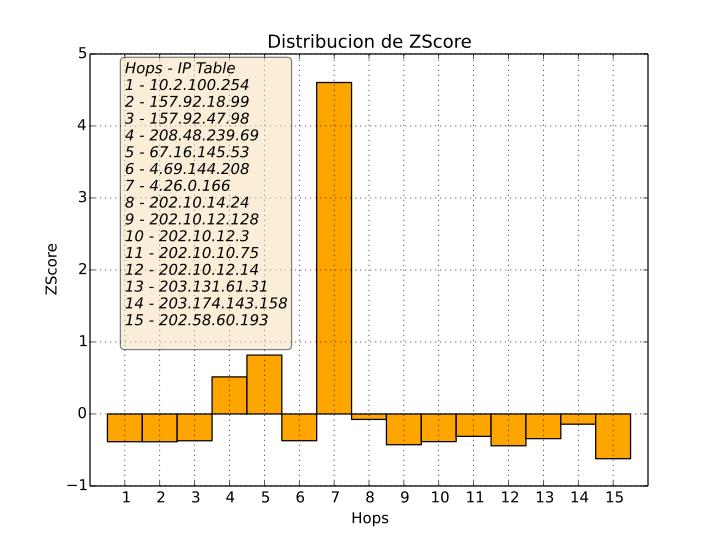
\includegraphics[scale=0.5]{../australia-experiment/bar_z_score.jpeg}
  \caption{Z-Score para cada uno de los saltos.}
	\label{fig:histo-src-sitiotrabajo}
\end{figure}

\subsubsection{Tabla de Hops de la traza}
\begin{center}
  \resizebox{\textwidth}{!}{\begin{tabular}{| c | c | c | c | c | c |}
		\hline
		Hop Score & Hop Ip & RTT Acum & RTT Incr & Hop Location & Hop Name\\
		\hline
		-0.385 & 10.2.100.254 & 0.35 & 0.35 & -,  & -\\
		\hline
		-0.386 & 157.92.18.99 & 0.63 & 0.28 & Argentina, Buenos Aires & ccc-pab2.fcen.uba.ar.\\
		\hline
		-0.372 & 157.92.47.98 & 1.43 & 0.8 & Argentina, Buenos Aires & -\\
		\hline
		0.515 & * & * & 32.758 & - & *\\
		\hline
		0.515 & * & * & 32.758 & - & *\\
		\hline
		0.515 & * & * & 32.758 & - & *\\
		\hline
		0.515 & 208.48.239.69 & 132.46 & 32.758 & United States, Lawrenceville & ethernet14-4.ar4.mia1.gblx.net.\\
		\hline
		0.818 & 67.16.145.53 & 176.14 & 43.68 & United States,  & po5.ar3.MIA2.gblx.net.\\
		\hline
		-0.371 & * & * & 0.825 & - & *\\
		\hline
		-0.371 & * & * & 0.825 & - & *\\
		\hline
		-0.371 & * & * & 0.825 & - & *\\
		\hline
		-0.371 & * & * & 0.825 & - & *\\
		\hline
		-0.371 & * & * & 0.825 & - & *\\
		\hline
		-0.371 & * & * & 0.825 & - & *\\
		\hline
		-0.371 & * & * & 0.825 & - & *\\
		\hline
		-0.371 & 4.69.144.208 & 182.74 & 0.825 & United States,  & ae-4-90.edge1.LosAngeles6.Level3.net.\\
		\hline
		4.604 & 4.26.0.166 & 362.88 & 180.14 & United States,  & AAPT-LIMITE.edge1.LosAngeles6.Level3.net.\\
		\hline
		-0.076 & 202.10.14.24 & 374.35 & 11.47 & Australia,  & po9.sclardist02.aapt.net.au.\\
		\hline
		-0.427 & 202.10.12.128 & 373.16 & -1.19 & Australia,  & te2-1-110.sclardist01.aapt.net.au.\\
		\hline
		-0.384 & 202.10.12.3 & 373.52 & 0.36 & Australia,  & bu11.sclarcore01.aapt.net.au.\\
		\hline
		-0.311 & 202.10.10.75 & 376.52 & 3 & Australia,  & bu1.mburncore01.aapt.net.au.\\
		\hline
		-0.442 & 202.10.12.14 & 374.8 & -1.72 & Australia,  & te2-2.mburndist01.aapt.net.au.\\
		\hline
		-0.343 & 203.131.61.31 & 376.63 & 1.83 & Australia, Melbourne & 1-1-1.mburninte01.aapt.net.au.\\
		\hline
		-0.142 & 203.174.143.158 & 385.73 & 9.1 & Australia, Adelaide & 203-174-143-158.ade.static-ipl.aapt.com.au.\\
		\hline
		-0.621 & * & * & -8.165 & - & *\\
		\hline
		-0.621 & 202.58.60.193 & 369.4 & -8.165 & Australia, Findon & -\\
		\hline
	\end{tabular}}
\end{center}

\subsubsection{Tabla de Hops Distinguidos}
\begin{center}
  \resizebox{\textwidth}{!}{\begin{tabular}{| c | c | c | c | c | c |}
		\hline
		Hop Score & Hop Ip & RTT Acum & RTT Incr & Hop Location & Hop Name\\
		\hline
		0.515 & *  & * & 32.758 & - & -\\
		\hline
		0.515 & *  & * & 32.758 & - & -\\
		\hline
		0.515 & *  & * & 32.758 & - & -\\
		\hline
		0.515 & 208.48.239.69 & 132.46 & 32.758 & United States, Lawrenceville  & ethernet14-4.ar4.mia1.gblx.net.\\
		\hline
		0.818 & 67.16.145.53 & 176.14 & 43.68 & United States,   & po5.ar3.MIA2.gblx.net.\\
		\hline
		4.604 & 4.26.0.166 & 362.88 & 180.14 & United States,   & AAPT-LIMITE.edge1.LosAngeles6.Level3.net.\\
		\hline
	\end{tabular}}
\end{center}

\subsubsection{Estadística sobre las mediciones de RTT incremental}
\begin{itemize}
	\item $\overline{RTT_i}: 14.208$
	\item $STDEV(RTT_i): 36.041$
\end{itemize}

\subsubsection{Conclusión y aclaraciones}
Podemos observar que el promedio del $RTT_i$ condice con el gráfico, y la desviacion estandar es alta, debido a la gran variacion del salto distinguido. En este caso particular tenemos varias aclaraciones que hacer. Para comenzar, tenemos dos resultados extraños, el primero, que el nodo distinguido marcado en el planisferio entre \texttt{157.92.47.98, Argentina, Buenos Aires} y \texttt{208.48.239.69, United States, Lawrenceville}, ve enmascarados 3 hops desconocidos, a los cuales se les calculo un RTT proporcional junto al hop de Estados Unidos. Esto no afecto la deteccion del salto entre el sur y el norte de America, pero quisimos aclararlo igualmente. Por otro lado, notemos que los saltos entre \textbf{4.69.144.208, United States, ae-4-90.edge1.LosAngeles6.Level3.net.},   \textbf{4.26.0.166, United States, AAPT-LIMITE.edge1.LosAngeles6.Level3.net.} y \textbf{202.10.14.24, Australia, po9.sclardist02.aapt.net.au.} arroja resultados extraños en la medicion del zscore. Todo parece indicar que el salto intercontinental esta entre los hosts \textbf{ae-4-90.edge1.LosAngeles6.Level3.net.} y \textbf{AAPT-LIMITE.edge1.LosAngeles6.Level3.net.} ambos ubicados en Estados Unidos, realizando una investigacion mas exhaustiva, encontramos que \texttt{AAPT Limited} es una gran compañia de telecomunicaciones de Australia, que se encarga de infraestructura, entre otras cosas, lineas submarinas. Nuestra suposicion acerca de este resultado es que el cable submarino entre \textbf{Estados Unidos} y \textbf{Australia} tiene IP de dominio estadounidense en ambos extremos del cable y el verdadero salto intercontinental se ve reflejado en el outlier del RTT incremental entre los hosts \textbf{ae-4-90.edge1.LosAngeles6.Level3.net.}, \textbf{AAPT-LIMITE.edge1.LosAngeles6.Level3.net.}.\\
Podemos ver finalmente que para este experimento, pudimos identificar los cables intercontinentales tanto con las herramientas de geolocalización como las herramientas estadísticas.

\subsection{www.cam.ac}

\subsection{home.web.cern.ch}

En este experimento se creo un paquete ICMP con dirección IP destino \textit{137.138.76.28}, correspondiente a la web \textit{http://home.web.cern.ch/} página oficial de la Organización Europea para la Investigación Nuclear (CERN). Los servidores de este sitio web se encuentran en la ciudad de Ginebra, Suiza. Se espera por lo tanto que a lo largo del camino que tome el paquete haya un salto transoceánico entre dos routers que obtendrá un alto puntaje según el z-score. Veamos primero una lista de las IPs junto a los lugares físicos asociados a esta para visualizar con mayor facilidad el recorrido que realizó el paquete a lo largo del experimento:

\begin{figure}[H]
  \centering	
	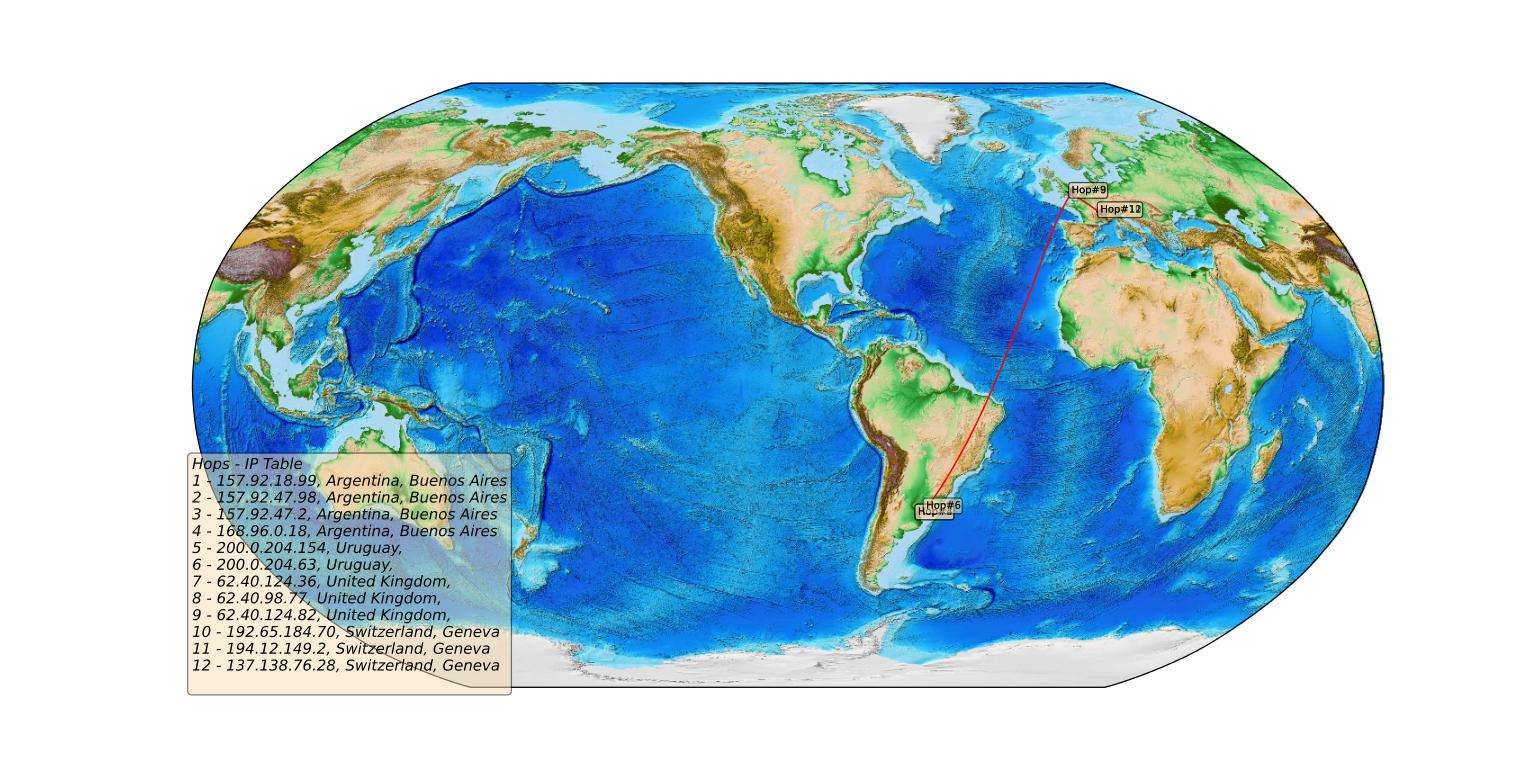
\includegraphics[scale=0.3]{../cern-experiment/figure_1.jpeg}
  \caption{Mapamundi con un croquis del viaje realizado por el paquete en rojo.}
	\label{fig:histo-src-sitiotrabajo}
\end{figure}

Como se puede ver el \textit{hop} entre el sexto y septimo router es el transoceánico del que se habló anteriormente. El salto se produce entre Uruguay (\textit{200.0.204.63}) y el Reino Unido (\textit{62.40.124.36}). En el siguiente gráfico, que muestra el RTT entre dos routers consecutivos medido en milisegundos, el salto que arriba al Reino Unido es el que devuelve el valor más alto. Esto tiene sentido ya que este es el de mayor distancia geográfica.

\begin{figure}[H]
  \centering	
	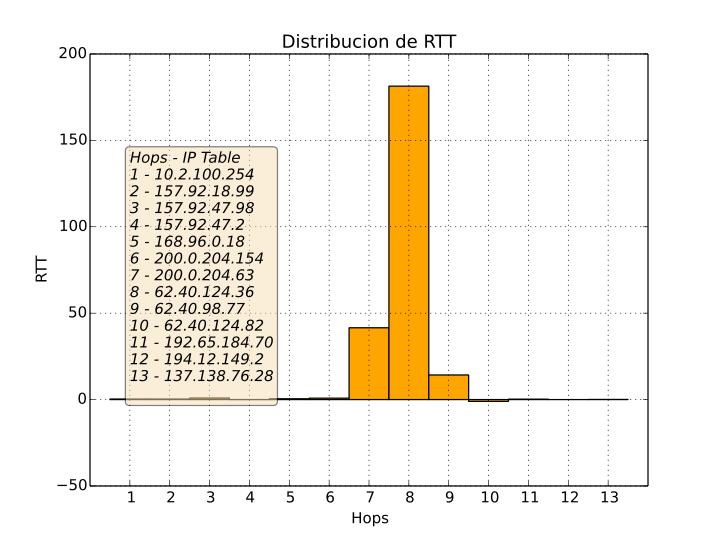
\includegraphics[scale=0.4]{../cern-experiment/bar_rtt.jpeg}
  \caption{RTT entre dos router consecutivos medido en milisegundos.}
	\label{fig:histo-src-sitiotrabajo}
\end{figure}

\begin{figure}[H]
  \centering	
	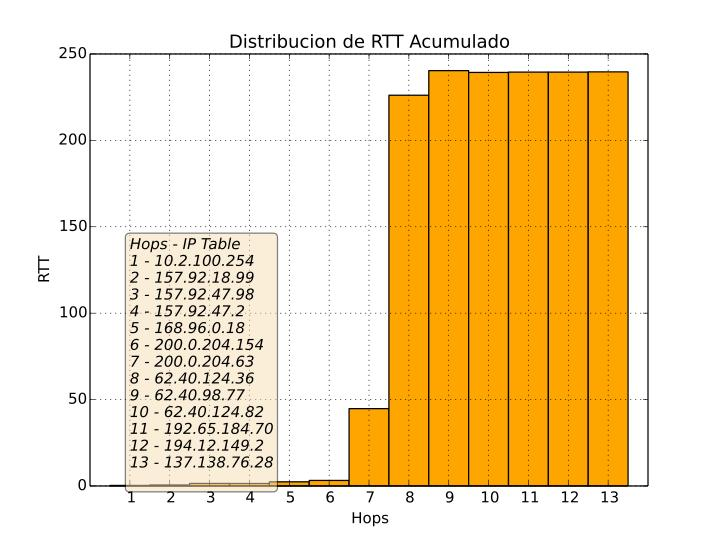
\includegraphics[scale=0.4]{../cern-experiment/bar_rtt_acum.jpeg}
  \caption{RTT acumulado del paquete a medida que avanza en su camino hacia el host del CERN.}
	\label{fig:histo-src-sitiotrabajo}
\end{figure}

Finalmente, se pueden ver los resultados obtenidos con el \textit{z-score} donde se observan valores similares (en proporción) a los obtenidos en el primer gráfico de esta sección. Más aun, el puntaje fue negativo para aquellos saltos que pueden ser etiquetados como de menor importancia, aquellos que tienen un desplazamiento geográfico menor y en consecuencia no aportan demasiado al tiempo total de viaje del paquete. Entre los saltos destacados, se puede ver una diferencia más pronunciada a la hora de encontrar al octavo como \textit{hop} distinguido.

\begin{figure}[H]
  \centering	
	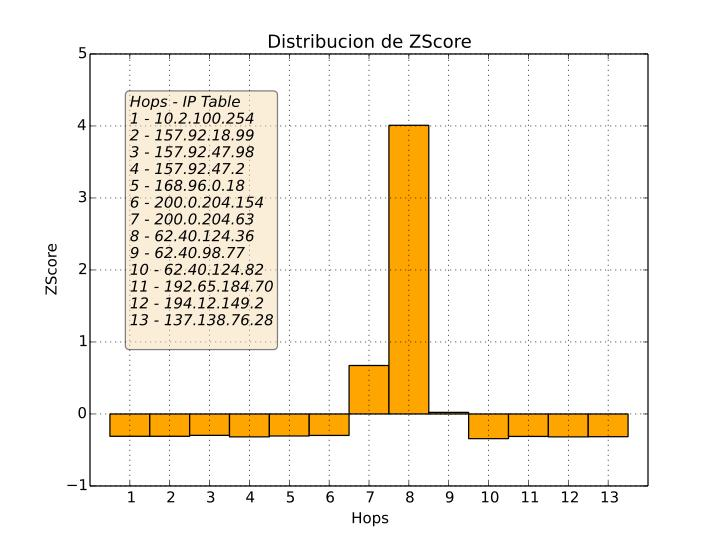
\includegraphics[scale=0.4]{../cern-experiment/bar_z_score.jpeg}
  \caption{Z-Score para cada uno de los saltos.}
	\label{fig:histo-src-sitiotrabajo}
\end{figure}

\section{Experimentaci\'on}

Como fue previamente mencionado, la idea ser\'a estudiar qu\'e par\'ametros optimizan el c\'alculo de RTO. Para realizar esto, dividiremos la experimentaci\'on en dos etapas.

Durante la primera etapa, analizaremos c\'omo evoluciona la estimaci\'on de RTO en el cliente con distintas combinaciones de $\alpha$ y $\mathcal{B}$ para un delay fijo y probabilidad de p\'erdida de paquetes nula. A partir de esta experimentaci\'on nos quedaremos con 4 combinaciones de $\alpha$ y $\mathcal{B}$ que a nuestro crtierio son los mejores para estimar el RTO.

Durante la segunda etapa, observaremos c\'omo se comportan las combinaciones anteriores. Para ello volveremos a analizar como evoluciona la estimaci\'on de RTO en el cliente pero, esta vez, iremos variando el delay y la probabilidad de p\'erdida de paquetes. 

\subsection{Etapa Inicial: Estimacion de $\alpha$ y $\beta$}
Con una probabilidad de error nula y un delay de 0.25 segundos, fijaremos los parametros \'optimos de la estimacion del RTO.
Explicar heatmap de los graficos (colores de las barras varian segun magnitud Z del grafico)

\subsubsection{Efectividad en la aproximacion del RTO y el Rtt Real}
	explicar normalizacion de valores y 1-valor
	...graficos 3d de las barras con los alfa y beta variados

\begin{figure}[H]
  \centering	
	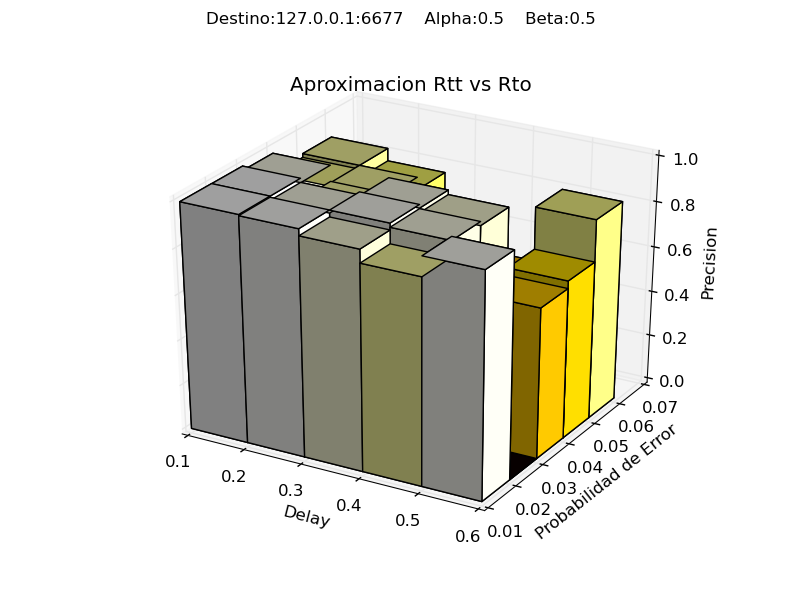
\includegraphics[scale=0.5]{../analisis/graficos_tablas/graficos_en_funcion_de_alfa_y_beta/graficos/rtt_vs_rto.png}
  \caption{Efectividad en la aproximaci\'on del RTO y el RTT Real en funci\'on de $\alpha$ y $\beta$}
	\label{fig:histo-src-sitiotrabajo}
\end{figure}

\subsubsection{Cantidad de retransmisiones}
	...graficos 3d de las barras con los alfa y beta variados

\begin{figure}[H]
  \centering	
	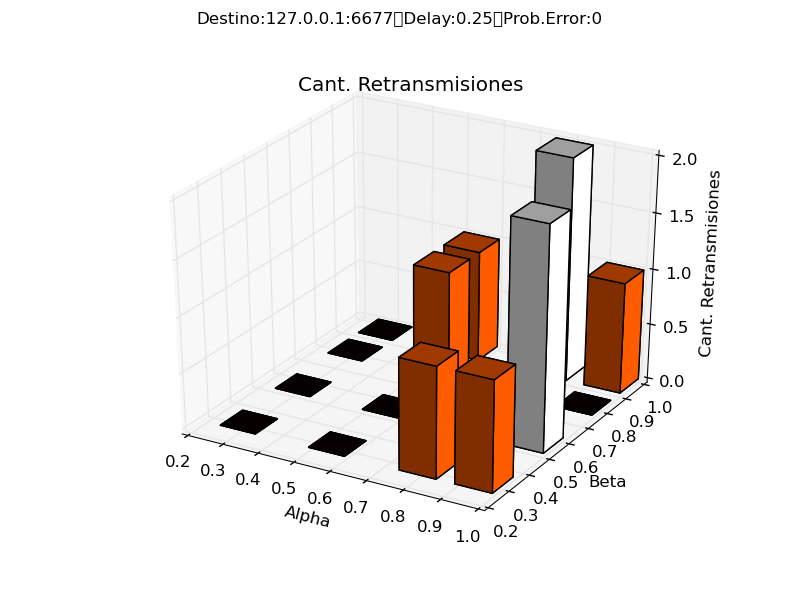
\includegraphics[scale=0.5]{../analisis/graficos_tablas/graficos_en_funcion_de_alfa_y_beta/graficos/retransmisiones.png}
  \caption{Retransmisiones en funci\'on de $\alpha$ y $\beta$}
	\label{fig:histo-src-sitiotrabajo}
\end{figure}

\subsubsection{RTO Estimado}
	...graficos 3d de las barras con los alfa y beta variados

\begin{figure}[H]
  \centering	
	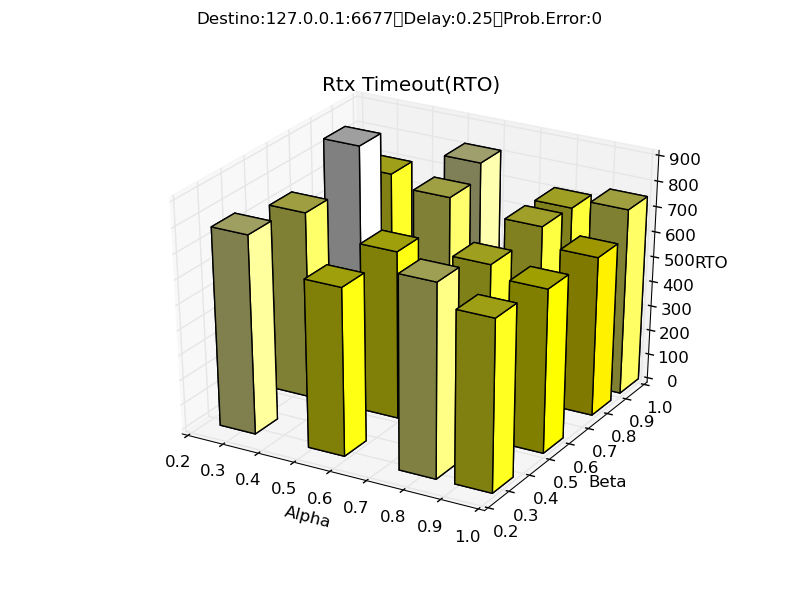
\includegraphics[scale=0.5]{../analisis/graficos_tablas/graficos_en_funcion_de_alfa_y_beta/graficos/rto.png}
  \caption{RTO en funci\'on de $\alpha$ y $\beta$}
	\label{fig:histo-src-sitiotrabajo}
\end{figure}

\subsection{Segunda Etapa - Simulacion de problemas de red: Delay y Errores inducidos con probabilidad}
\section{Experimentacion Adicional}
De ciertas experimentaciones adicionales realizadas por curiosidad pero no presentadas en este informe dado el alcance del trabajo obtuvimos resultados extraños, como servidores de ISP intermedios contestando \texttt{Echo Reply} como si fueran el host destino, creemos que esto se debe a un cacheo intermedio que realiza el ISP para minimizar la redireccion de trafico fuera del pais. Otros experimentos realizados sobre la red movil 3g anclando la conexion a una pc, mostraron una cantidad de saltos muy grande dentro del pais, con tiempos de \texttt{Round Trip Time} muy altos en comparacion al enlace submarino hasta el host destino, los nodos distinguidos de la ruta quedaron enmarcados dentro del pais, lo cual podria explicarse por el nivel de congestion de la red de telefonia de la capital. Otros experimentos realizados sobre redes 3G arrojan una cantidad innecesaria de hops entre continentes para llegar a destino, particularmente los paquetes iban de Argentina, a Uruguay, luego a Italia, luego a Estados Unidos, volvian al Reino Unido, y finalmente a destino en europa.\\
Algunos de los datos de los experimentos mencionados pueden encontrarse en el comprimido adjunto por fuera del informe.
\section{Conclusiones}
Como conclusion del trabajo pudimos entender como funciona el protocolo ICMP para realizar una traza con ttl incrementales, y obtener una buena aproximacion de los enlaces submarinos utilizando las herramientas desarrolladas en el trabajo. Los resultados fueron variados, en la seccion de \texttt{Experimentos Adicionales} se mencionan algunos resultados curiosos. En general es interesante la cantidad de datos, nombres de hosts y geograficos que pueden obtenerse a partir de la realizacion de una traza. Tambien son interesantes las aplicaciones practicas de las trazas, los datos obtenidos pueden utilizarse para diagnostico, por ejemplo se quiere saber en que momento se pierde un paquete, con la traza puede saberse en que hop se pierde. Otra posible aplicacion podr\'ia ser para aumentar la performance en el diseño de agregacion de enlaces adicionales a internet, alivianando la carga en los hops con mucho \texttt{RTT incremental}.


\end{document}
